\documentclass[020-persona\_validation.tex]{subfiles}

\begin{document}

\subsection{Pre-Workshop Student Self-Assessment Survey (Persona Survey) Supplemental Factor Analysis Results}
\label{sse:persona-survey-supplemental-results}

    \begin{figure}[!hbtp]
        \centering
        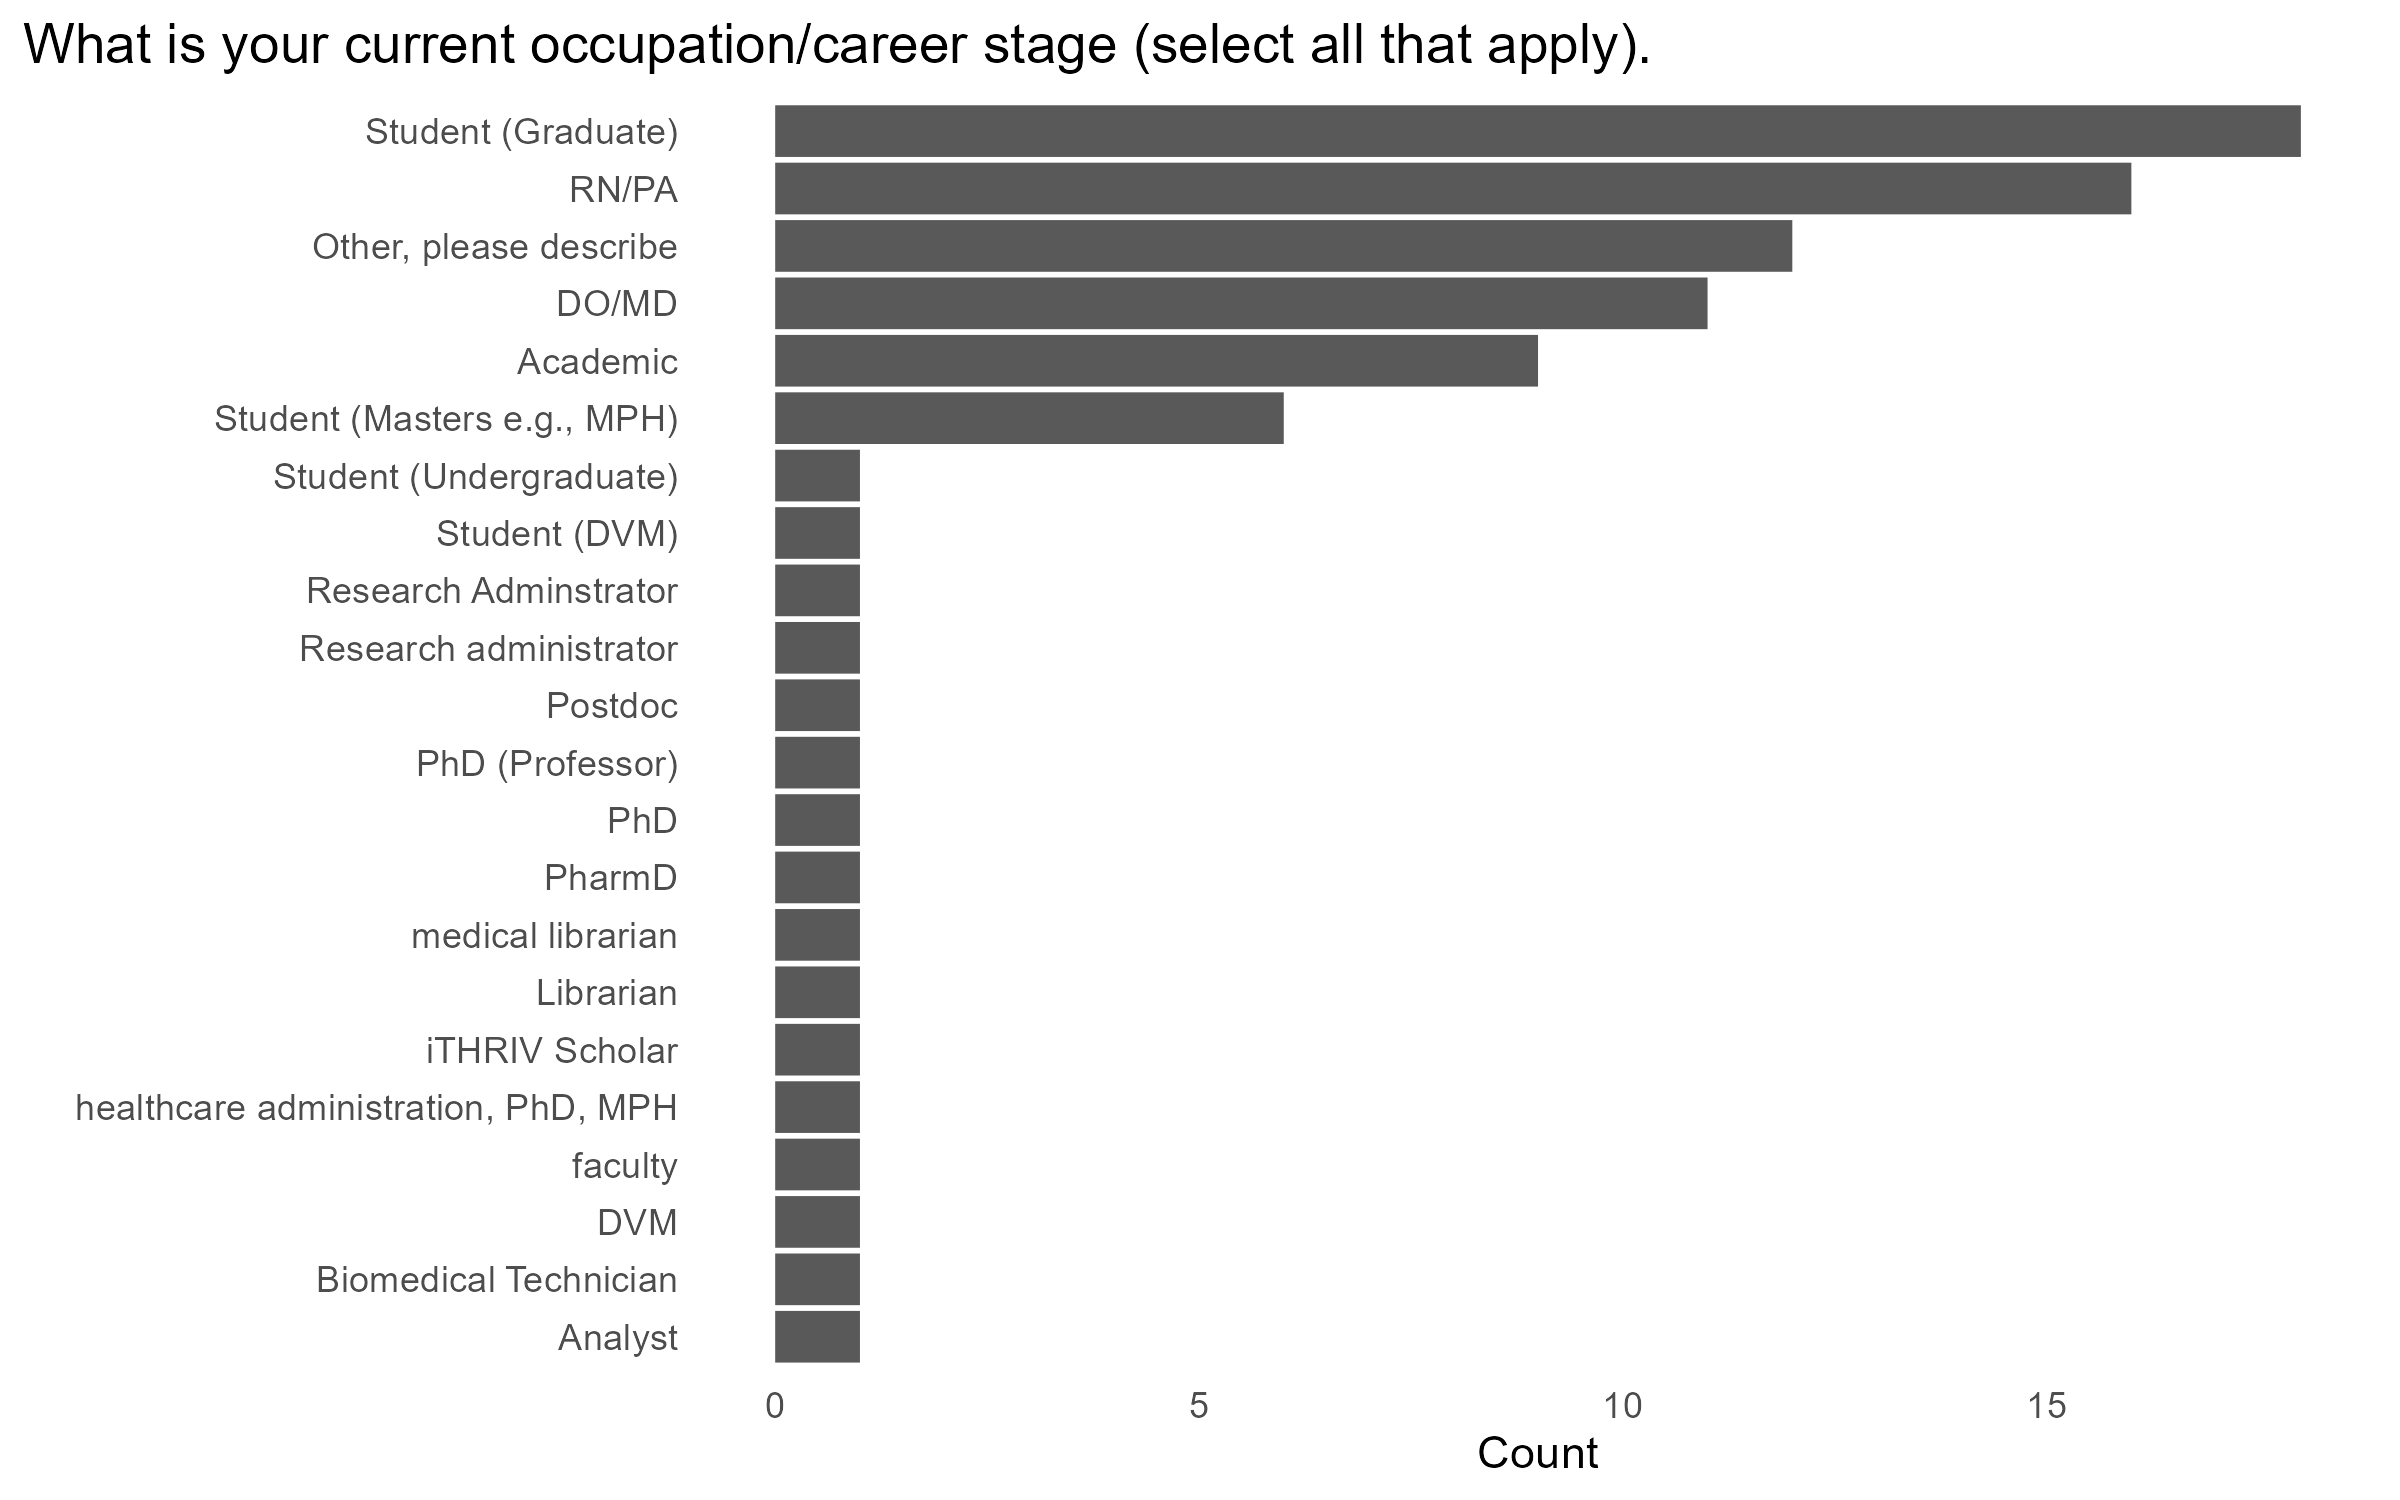
\includegraphics[width=0.7\linewidth]{figs/020-persona/Q2.3.png}
        \caption[What is your current occupation/career stage (select all that apply)]
        {Self reported current occupation and career stage.
            Respondents are able to select multiple options and also write in their own choices.
        }
        \label{fig:demographics_occupation}
    \end{figure}

    \begin{figure}[!hbtp]
        \centering
        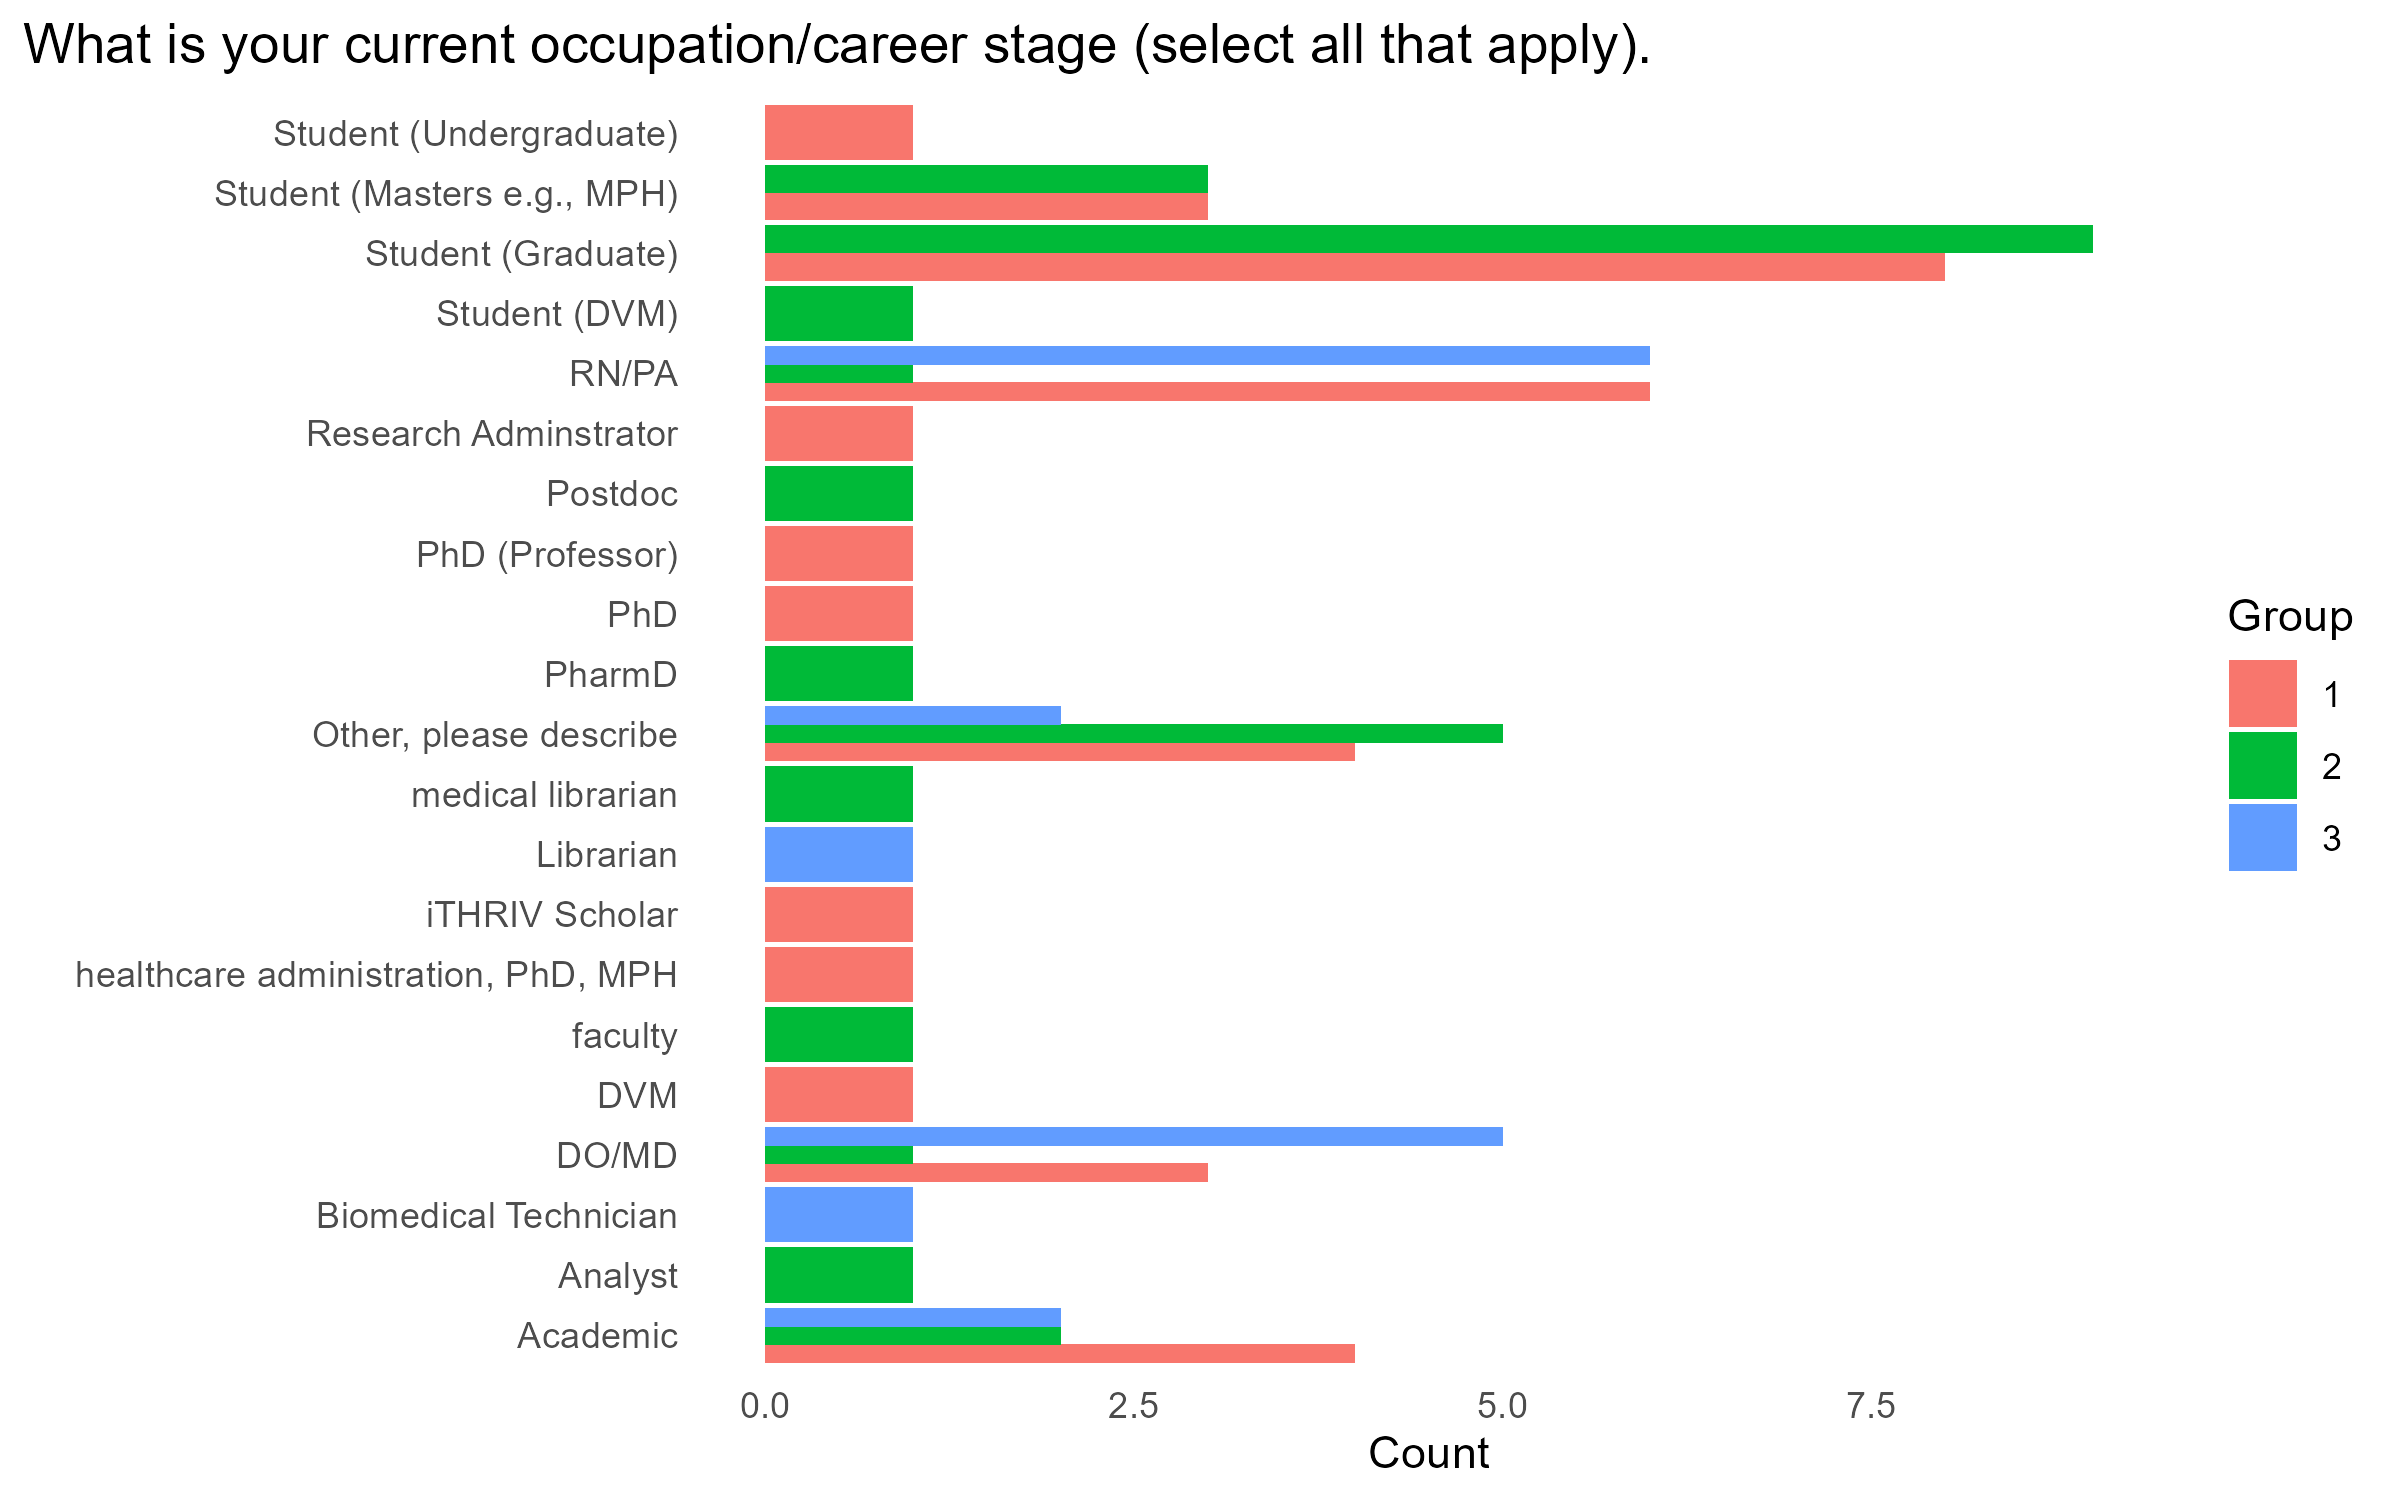
\includegraphics[width=0.7\linewidth]{figs/020-persona/survey\_likert/Q2.3-group-3.png}
        \caption[What is your current occupation/career stage by group (select all that apply)]
        {Self reported current occupation and career stage by clustering group.
            Respondents are able to select multiple options and also write in their own choices.
        }
        \label{fig:demographics_occupation_cluster}
    \end{figure}

    \begin{figure}[!hbtp]
        \centering
        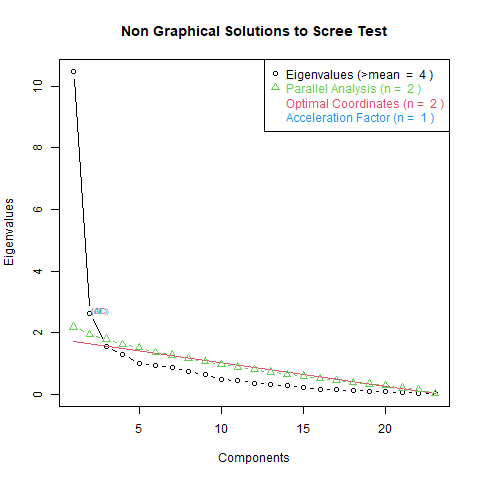
\includegraphics[scale=0.5]{figs/010-validation/efa_eigen_scree.png}
        \caption[Scree plot for factor analysis]i
        {Scree plot for factor analysis showing the number of components (x) and the eigenvalues (y) for all 23 survey items.
            The figure suggests exploring 2 to 4 factor models.
        }
        \label{fig:scree-fa-all}
    \end{figure}

    \begin{figure}[!hbtp]
        \centering
        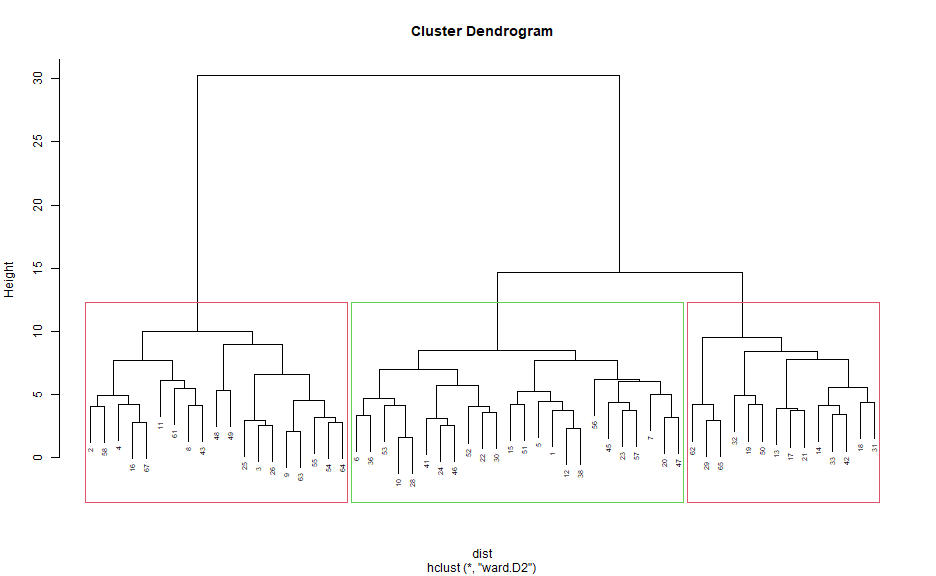
\includegraphics[width=0.9\linewidth]{figs/020-persona/survey\_likert/dendogram_3.png}
        \caption[Dendrogram of the 3 learner persona clusters]
        {Dendrogram of the three (3) learner persona clusters.
        The clusters were combined with the survey responses to identify the learner personas.
        From left to right, the clusters are: Samir Student (Group 2), Alex Academic (Group 1),
        and Clare Clinician (Group 3).
        }
        \label{sfig:dendro-cluster-3}
    \end{figure}

    \begin{figure}[!hbtp]
        \centering
        \includegraphics[width=0.9\linewidth]{figs/020-persona/survey\_likert/dendogram\_4.png}
        \caption[4 cluster Dendrogram.]
        {Dendrogram showing 4 clusters. Looking at the differences in how the clusters were split from the 3-cluster model
        (Figure \ref{sfig:dendro-cluster-3}),
        the same group that eventually was named Samir Student (Group 2) was split into another cluster.
        This split was hard to interpret, so the 3-cluster model was used for creating the learner personas.
        }
        \label{sfig:dendro-4}
    \end{figure}

    \begin{figure}[!hbtp]
        \centering
        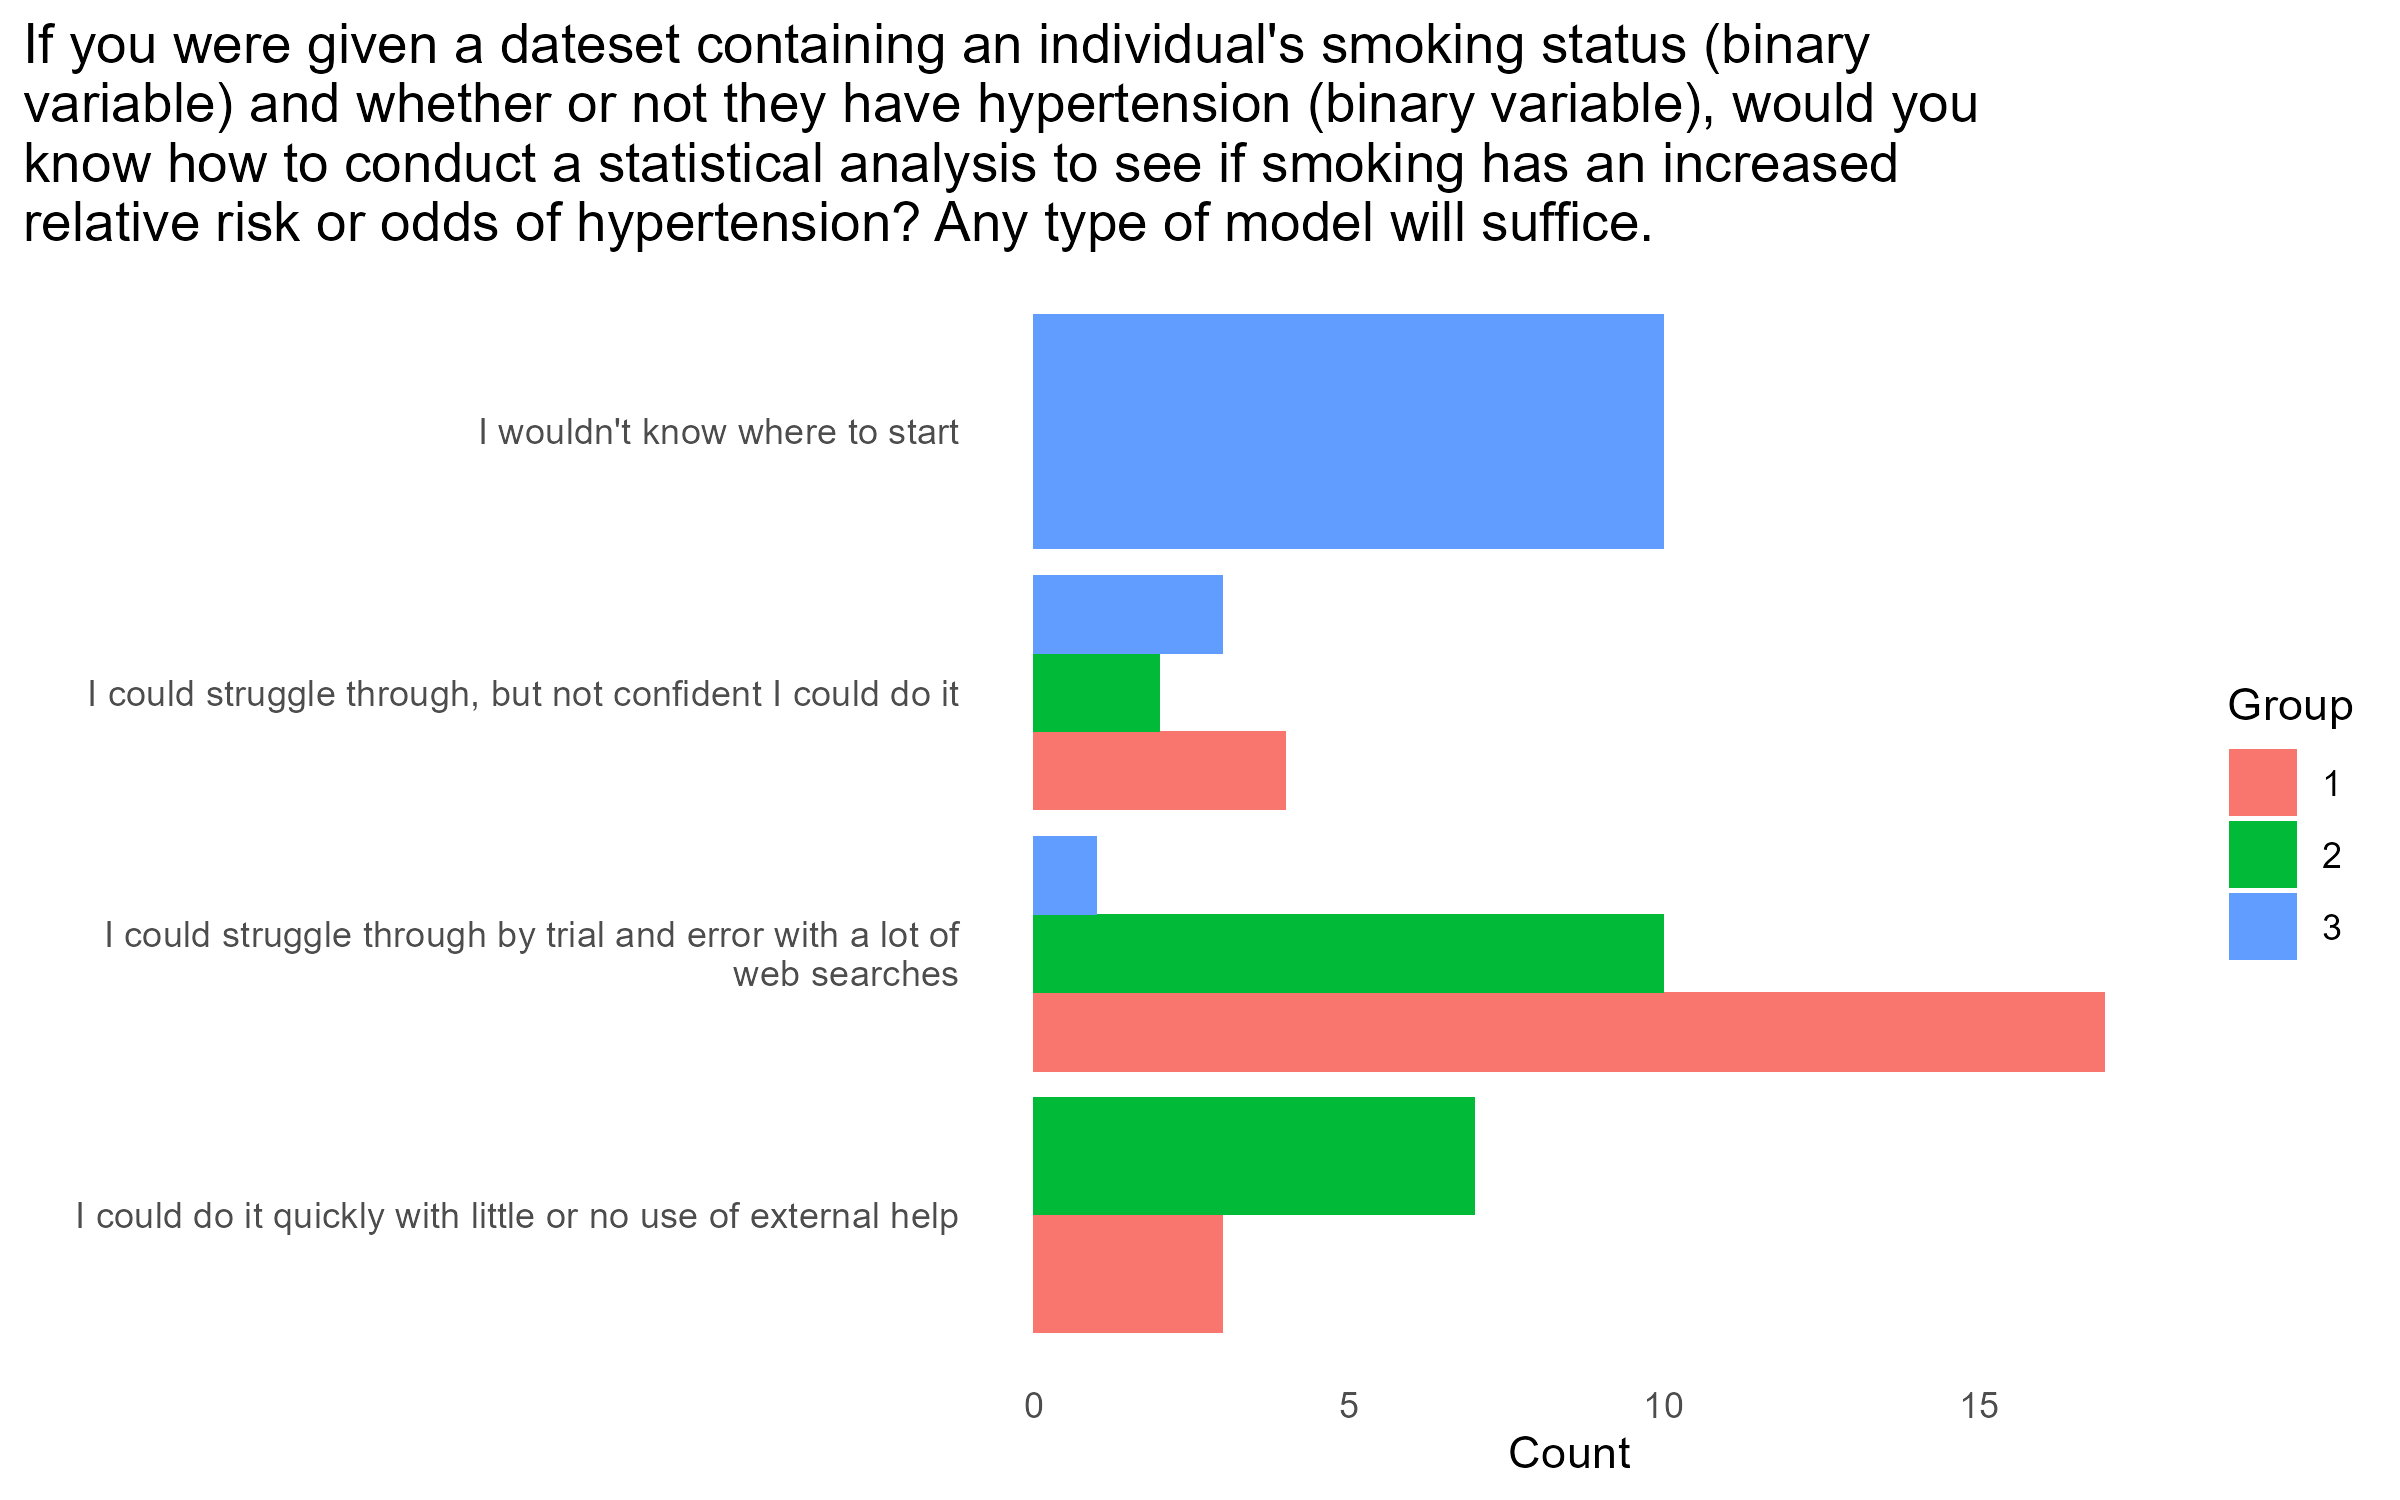
\includegraphics[width=0.9\linewidth]{figs/020-persona/survey\_likert/Q6.2-group-3.png}
        \caption[Q6.2: Statistics question result for 3 clusters]
        {Participants were asked if they were able to perform an analysis with a binary outcome.
            The full question asked
            ``If you were given a dataset containing an individual's smoking status (binary variable)
            and whether or not they have hypertension (binary variable),
            would you know how to conduct a statistical analysis
            to see if smoking has an increased relative risk or odds of hypertension? Any type of model will suffice.''
            Typically, logistic regression would be performed for this kind of problem,
            but the authors were less concerned with identifying a particular analysis,
            and more focused if participants could perform any analysis.
            Group 3 were the only group that would not know how to start this kind of analysis,
            and also leaned towards struggling through this kind of analysis.
            Groups 1 and 2 leaned towards being able to perform this analysis task,
            with Group 2 having the most responses for performing the task with minimal external help.
            Group 2 also had a high number of responses for completing the task with some struggle,
            but Group 1 had the most frequent number of responses.
        }
        \label{sfig:cluster-q6-2}
    \end{figure}

    \begin{figure}[!hbtp]
        \centering
        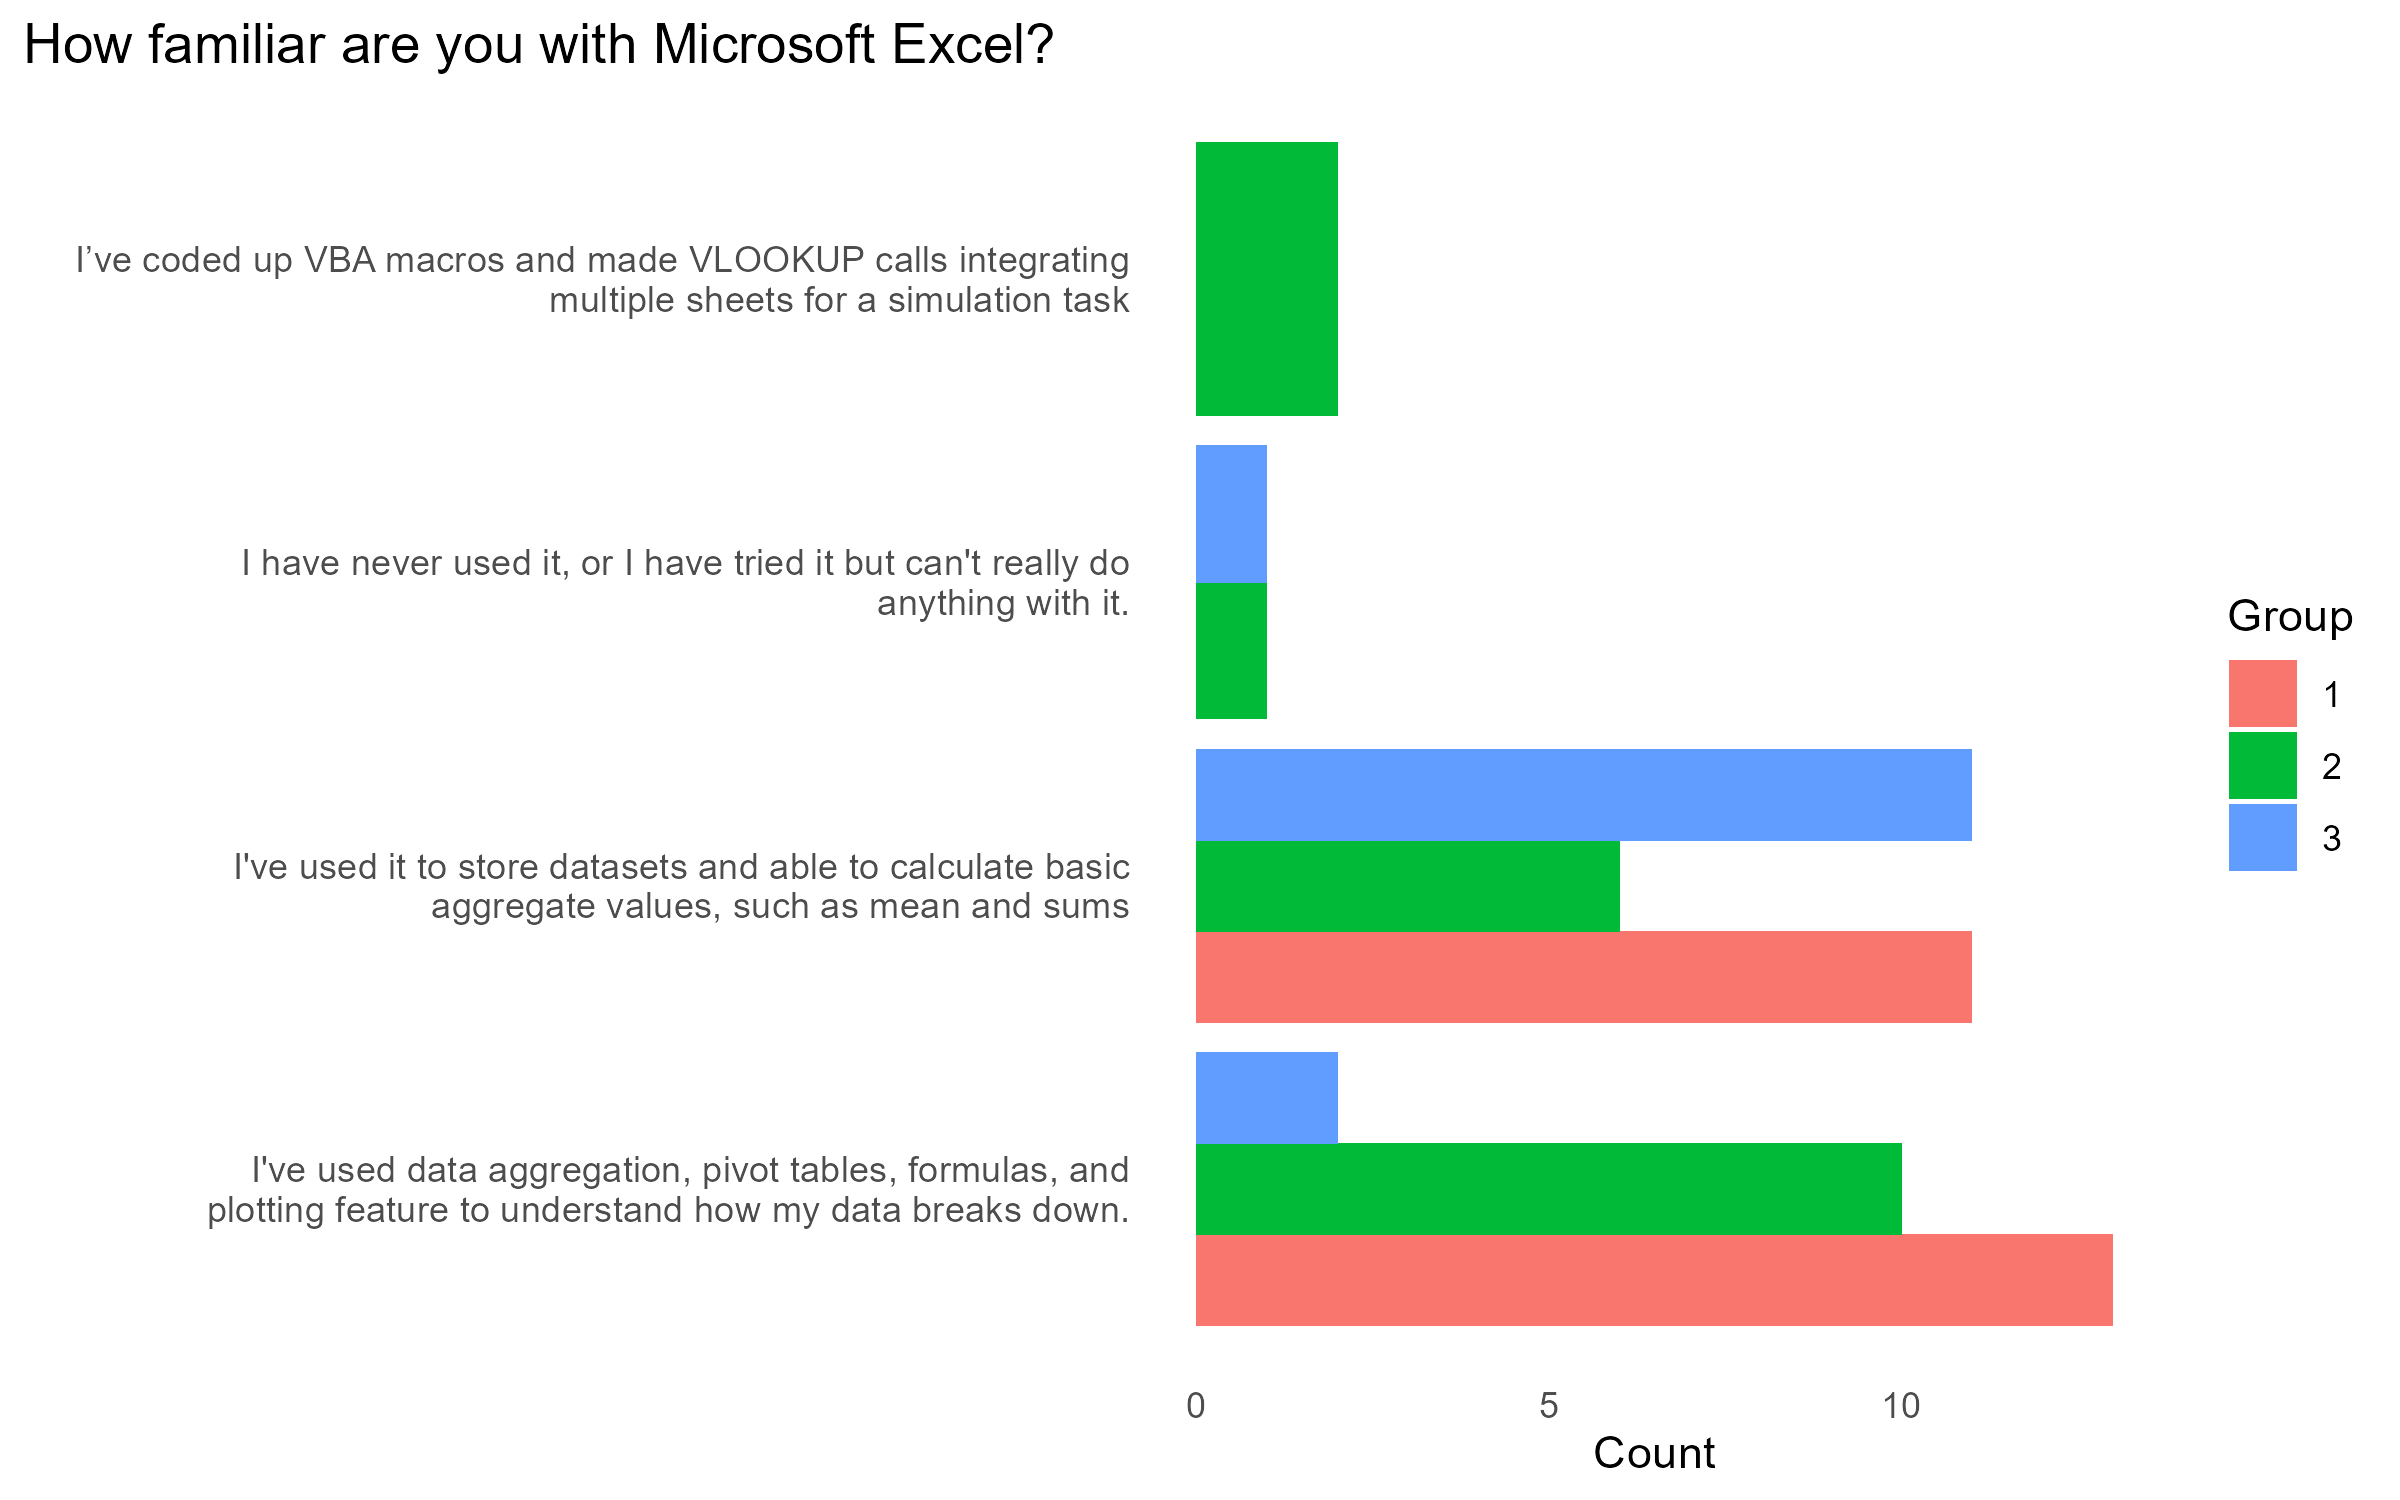
\includegraphics[width=0.9\linewidth]{figs/manual\_copy/Q4.1.png}
        \caption[Q4.1: Excel proficiency across 3 clusters]
        {Participants were asked about their familiarity with Microsoft Excel.
            The full question asked
            ``How familiar are you with Microsoft Excel''?
            The responses showed that many of the respondents how how to use Excel for basic data tasks and calculations,
            and very few of the respondents were highly proficient in using Excel for data tasks.
        }
        \label{sfig:cluster-q4.1}
    \end{figure}


\end{document}
